\chapter*{Annexe 1}
\addcontentsline{toc}{chapter}{Annexe 1}
\newtheorem{kkk}{Théorème}

%changer le format des sections, subsections pour apparaittre sans le num de chapitre
\makeatletter
\renewcommand{\thesection}{\@arabic\c@section}
\makeatother

%recommencer la numérotation des section à "1"
\setcounter{section}{0}

\begin{kkk}(Axiome du choix)
  \hfill

\noindent
  Pour tout ensemble $X$ d'ensembles non vides, il existe une fonction définie sur $X$, appelée fonction de choix, qui à chaque ensemble $A$ appartenant à $X$ associe un élément de cet ensemble.
  \label{axiome}
\end{kkk}

\begin{kkk}(Théorème de Wallace-Bolyai-Gerwien)\label{wbg}
  \hfill

\noindent
Pour que deux polygones du plan aient la même aire, il faut et il suffit qu'ils soient équivalents par découpage fini.
\end{kkk}
\begin{proof}
  \hfill
  \begin{itemize}
    \item On commence par découper le premier polygone en triangles. Considérons le sommet le plus à gauche du polygone, $P_3$ sur la figure suivante, et le segment formé des deux sommets voisins $P_2$ et $P_4$, si ce dernier est inclu dans le polygone alors Le triangle $P_2P_3P_4$ peut être ajouté à la liste des triangles qui composent le polygone. Le sommet $P_3$ est enlevé du polygone, et on applique récursivement la triangulation au polygone restant $P_0P_1P_2P_4P_5P_6$.
    \begin{figure}[h]
        \centering
        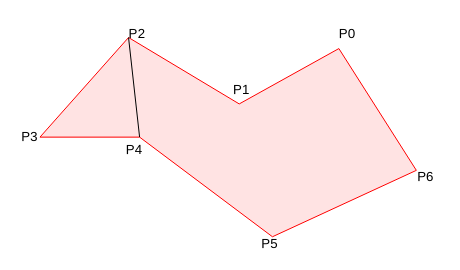
\includegraphics[scale=0.6]{images/x5.png}

        % \caption{Une représentation graphique d'un groupe libre de rang 2}
    \end{figure}

    sinon si le segment formé des deux sommets voisins n'est pas à l'intérieur du polygone, il existe nécessairement un ou plusieurs sommets à
l'intérieur du triangle $P_2P_3P_4$. Soit $P_j$ le sommet situé dans le triangle $P_2P_3P_4$ le plus loin de $P_2P_4$. Le segment $P_3P_j$ est à l'intérieur du polygone, car si un côté coupait ce segment, il aurait une extrémité dans le triangle $P_2P_3P_4$, plus éloigné de $P_2P_4$ que $P_j$.\\ La diagonale $P_3P_j$ permet de diviser le polygone initial en deux polygones. On applique récursivement la diagonalisation à ces deux polygones.

    \begin{figure}[h]
        \centering
        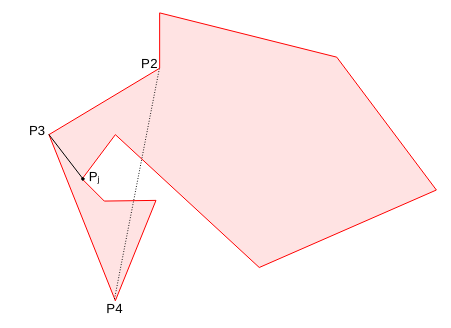
\includegraphics[scale=0.6]{images/x6.png}

        % \caption{Une représentation graphique d'un groupe libre de rang 2}
    \end{figure}
    \newpage
    \item Après, on transforme chaque triangle en un rectangle (ce découpage s'applique à tout triangle, car dans tout triangle au moins l'une des hauteurs coupe le côté opposé)
    \begin{figure}[h]
        \centering
        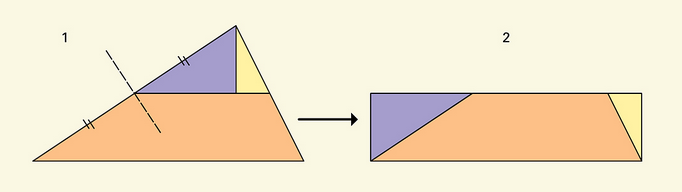
\includegraphics[scale=0.6]{images/x1.png}

        % \caption{Une représentation graphique d'un groupe libre de rang 2}
    \end{figure}
    \item Si le rectangle a une longueur supérieur à quatre fois sa largeur on le découpe en deux (en longueur) et on le réarange de la manière suivante

    \begin{figure}[h]
        \centering
        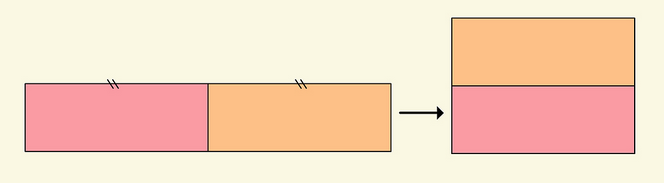
\includegraphics[scale=0.6]{images/x2.png}

        % \caption{Une représentation graphique d'un groupe libre de rang 2}
    \end{figure}

    et on répète cette opération jusqu'à obtenir un rectangle dont la longueur est inférieur à quatre fois sa largeur.
    \item On transforme chaque rectangle en carré de la manière suivante
    \newpage

    \begin{figure}[h]
        \centering
        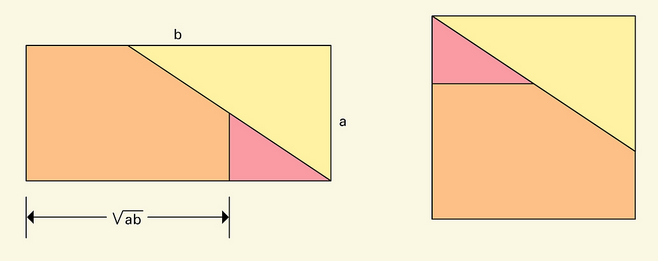
\includegraphics[scale=0.6]{images/x3.png}

        % \caption{Une représentation graphique d'un groupe libre de rang 2}
    \end{figure}

    ceci est possible si et seulement si $\sqrt{ab} \ge b-\sqrt{ab}$ c'est à dire si et seulement si $b \le 4a$.
    \item On fusionne les carrés, deux par deux, progressivement, jusqu'à avoir un unique grand carré de la manière suivante
    \begin{figure}[h]
        \centering
        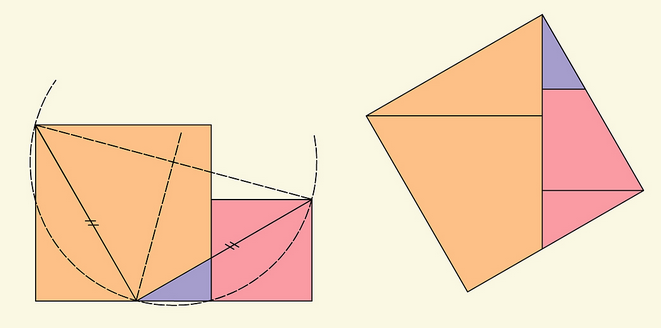
\includegraphics[scale=0.6]{images/x4.png}

        % \caption{Une représentation graphique d'un groupe libre de rang 2}
    \end{figure}
    \item On refait la même chose pour le deuxième polygone et on superpose les découpages intervenus pour transformer le polygone 1 en carré à ceux obtenus pour transformer le polygone 2 en carré. Par construction, les pièces résultantes permettent de reconstituer le polygone 1 et le polygone 2.
  \end{itemize}

\end{proof}
